%!TEX program = xelatex
\documentclass{article}
\usepackage[UTF8]{ctex}
\usepackage{blindtext}
\usepackage{graphicx}
\usepackage{epsfig}
\usepackage{float}
\usepackage[framemethod=TikZ]{mdframed}
\usepackage{url}   % 网页链接
\usepackage{subcaption} % 子标题
\usepackage{geometry}
\geometry{a4paper,left=3.17cm,right=3.17cm,top=2.54cm,bottom=2.54cm}
\title{1978 年至 2018 年中国居民人均可支配收入和支出的数学模型}
\author{吴承宇 20230616 \and 刘湑渊 20230610 \and 叶泽宇 20230621 \and 吴可悠 20230617}
\date{2023 December}
\begin{document}
\maketitle
\section*{摘要}
\begin{mdframed}
\fangsong
改革开放以来, 我国经济持续增长, 人民生活水平不断提高. 人均收入水平是一个重要的宏观经济指标, 也是衡量一个国家经济发展水平的重要指标. 本文通过建立线性回归模型, 分析了从 1978 年至 2018 年中国居民人均可支配收入和支出的数据, 并且预测了未来的发展趋势.\\
\end{mdframed}
\section*{关键词}
\begin{mdframed}
\fangsong
数学模型 \quad 中国经济 \quad 居民收入 \quad 居民支出 \quad 线性回归
\end{mdframed}
\section{问题背景}
改革开放以来, 中国经济发展迅速, 居民收入和支出也随之增长. 本文将对 1978 年至 2018 年中国居民人均可支配收入和支出的数据进行分析, 建立数学模型, 预测未来的发展趋势.\\
\indent 改革开放以来中国经济发展的客观因素主要有: 对外开放程度的扩大, 人口红利的释放, 以及自 2001 年加入世界贸易组织后, 中国经济与世界经济的深度融合.\\
\indent 中国共产党的领导对于改革开放的成功起到了决定性的作用. 中国共产党的领导使得中国能够在改革开放的过程中保持社会稳定, 从而使得改革开放能够顺利进行.\\
\indent 本文通过建立线性回归模型, 分析了从 1978 年至 2018 年中国居民人均可支配收入和支出的数据, 并且对于城镇和乡村进行线性比较. 本文的具体安排如下:
\begin{itemize}
    \item 第 2 节, 对于数据进行了分析, 通过绘制散点图, 分析了数据的分布规律.
    \item 第 3 节, 通过建立线性回归模型, 对于数据进行了分析, 并且预测了未来的发展趋势.
    \item 第 4 节, 对于题目所给出的问题进行了解答.
    \item 第 5 节, 对于城镇和乡村的数据进行了分析, 并且对于城镇和乡村的数据进行了线性比较.
    \item 第 6 节, 对于模型的优缺点进行了分析, 并且对于模型的改进进行了讨论.
\end{itemize}
\section{数据分析}\label{sec:analysis}
通过对于数据绘制散点图 (见图 1, 图 2), 可以发现数据的分布规律.\\
\begin{figure}[H]
  \centering
  \begin{minipage}[t]{0.48\textwidth}
    \centering
    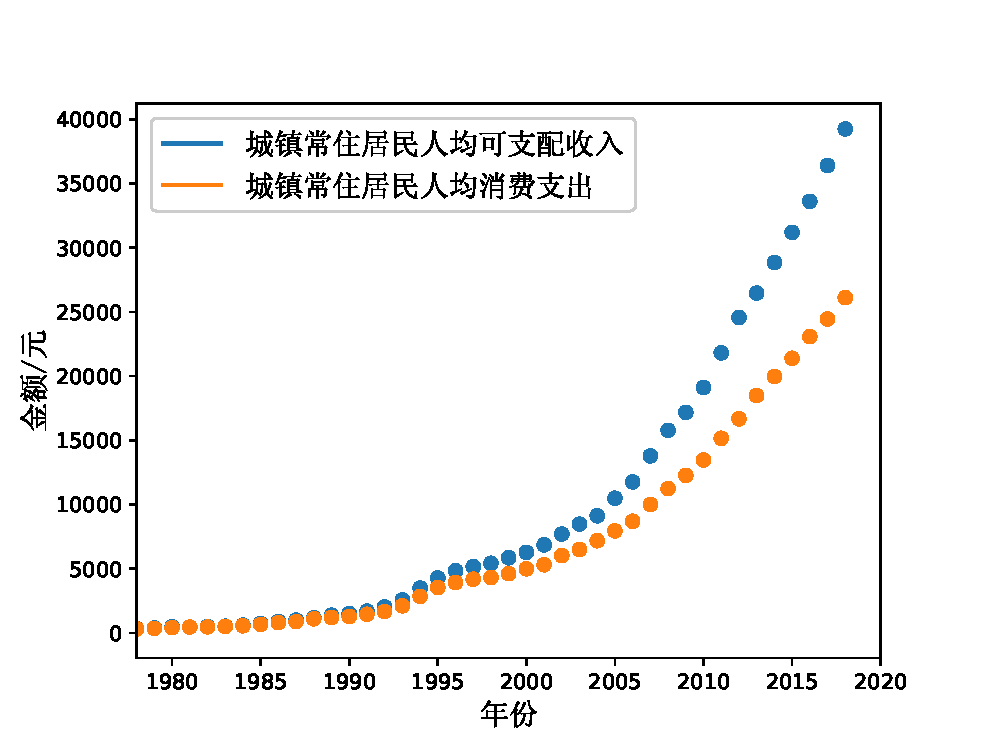
\includegraphics[width=0.8\textwidth]{figures/plot2.eps}
    \caption{城镇可支配收入和支出散点图}
    \label{fig:side:a}
  \end{minipage}
  \begin{minipage}[t]{0.48\textwidth}
    \centering
    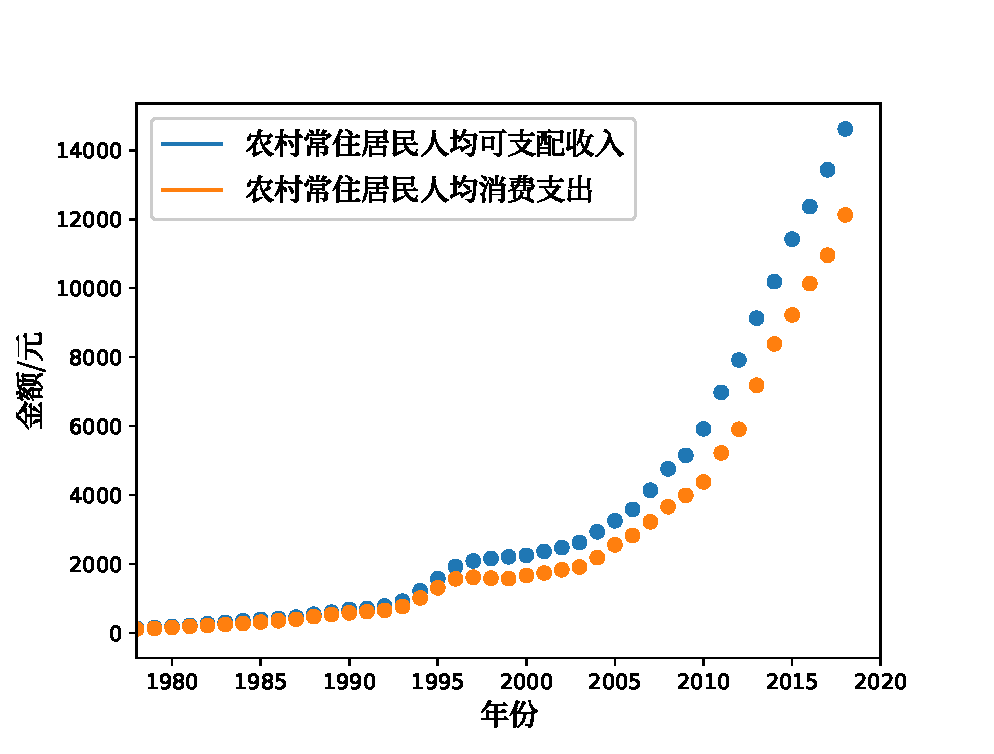
\includegraphics[width=0.8\textwidth]{figures/plot3.eps}
    \caption{乡村可支配收入和支出散点图}
    \label{fig:side:b}
  \end{minipage}
\end{figure}
通过图 \ref{fig:side:a} 和图 \ref{fig:side:b} 可以发现, 从 1978 年至 2018 年, 中国居民人均可支配收入和支出主要呈现指数增长的趋势.\\
\indent 整体而言, 收入增长速度大于支出增长速度, 且城镇的差值增长速度大于乡村.\\
\indent 同时, 将图 \ref{fig:side:a} 和图 \ref{fig:side:b} 叠加在一起 (见图 \ref{fig:side:c}), 可以发现城镇和乡村的数据分布规律基本相同, 但是城镇的增长速度明显快于乡村, 并且随着时间的增长, 差距越来越大.\\
\begin{figure}[H]
  \centering
  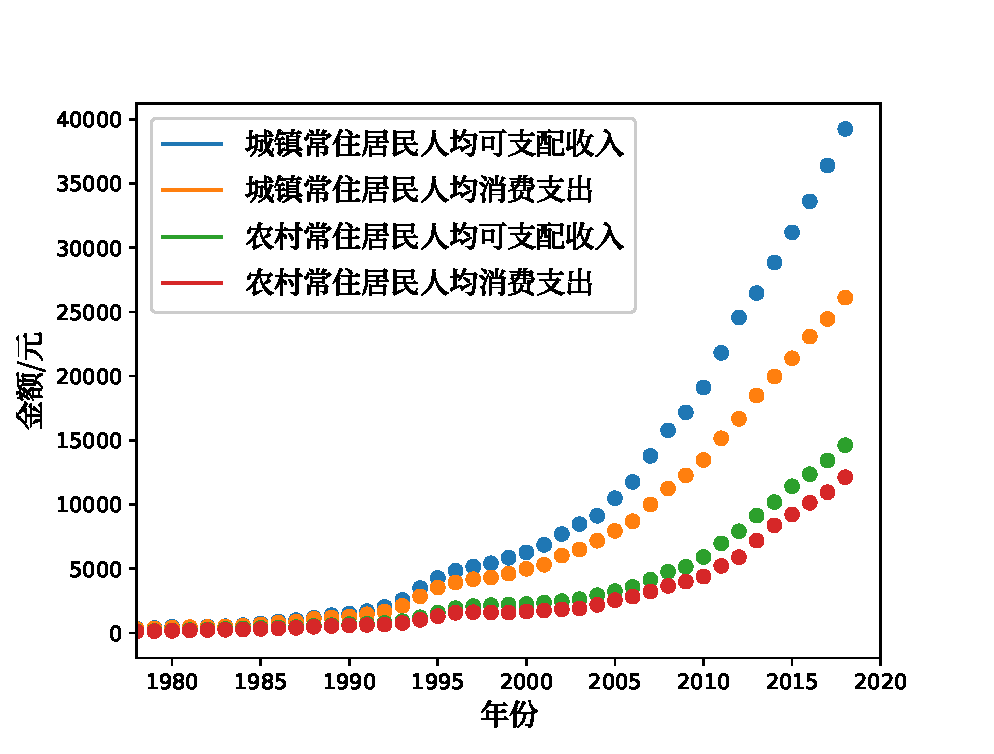
\includegraphics[width=0.8\textwidth]{figures/plot1.eps}
  \caption{可支配收入和支出散点图}
  \label{fig:side:c}
\end{figure}
从图 \ref{fig:side:c} 中可以发现, 城镇人均可支配收入和消费支出的数值首先与乡村持平, 随着时间的推移, 城镇的数值逐渐超过乡村, 并且差距越来越大.\\
\section{模型建立与分析}\label{sec:model}

\subsection{假设条件}

\begin{itemize}
  \item 假设居民人均可支配收入和支出的增长速度为指数增长.
  \item 假设没有其他因素影响居民人均可支配收入和支出的增长速度.
  \item 假设中国在未来的发展中, 经济发展的速度不会发生剧烈的变化.
\end{itemize}

\subsection{模型建立}
笔者使用线性回归分析的方法, 建立了居民人均可支配收入和支出的数学模型 (公式 \ref{eq:1}).\\
\indent 通过如下的模型, 分别对于城镇人均可支配收入, 城镇人均消费支出, 乡村人均可支配收入, 乡村人均消费支出进行线性回归分析:

\begin{equation}
  \label{eq:1}
  y=\theta_0e^{\theta_1\left(x-1978\right)}
\end{equation}

\indent 通过自然对数 $e$ 的幂函数, 可以将指数函数转化为线性函数, 从而使用线性回归分析的方法进行分析.\\
\indent 通过使用 \texttt{Python} 的 \texttt{sklearn} 库, 笔者得到了如下的结果:

\begin{table}[H]
  \centering
  \caption{线性回归分析结果}
  \label{tab:1}
  \begin{tabular}{cccccc}
    \hline
    \textbf{数据} & \textbf{$\theta_0$} & \textbf{$\theta_1$} & \textbf{loss} & \textbf{误差率} & \textbf{表达式} \\
    \hline
    城镇可支配收入 & 359.939478 & 0.124215 & 0.98911883 & 1.088\% & $y=359.939478e^{0.124215\left(x-1978\right)}$ \\
    城镇消费支出 & 345.872895 & 0.114970 & 0.98795625 & 1.204\% & $y=345.872895e^{0.114970\left(x-1978\right)}$ \\
    乡村可支配收入 & 173.015491 & 0.112898 & 0.99034022 & 1.066\% & $y=173.015491e^{0.112898\left(x-1978\right)}$ \\
    乡村消费支出 & 145.093811 & 0.110557 & 0.98983601 & 1.016\% & $y=145.093811e^{0.110557\left(x-1978\right)}$ \\
    \hline
  \end{tabular}
\end{table}

\indent 通过对于数据进行线性回归分析, 可以发现, 误差率都在 $1\%$ 以左右, 因此模型的拟合效果较好.\\

\subsection{模型分析}

\indent 通过对于模型的分析, 可以发现, 从 1978 年至 2018 年, 中国居民人均可支配收入和支出主要呈现指数增长的趋势.\\
\indent 整体而言, 收入增长速度大于支出增长速度, 且城镇的差值增长速度大于乡村. 从数据上, 城镇的两个数据的系数值 ($\theta_0$) 都约等于乡村的两个数据的系数值的 $2$ 倍. 同时, 城镇的两个数据的指数值 ($\theta_1$) 都约等于乡村的两个数据的指数值.\\
\indent 通过对于数据模型的建立, 笔者发现和先前观察散点图的结果大致相同, 但是对于起始的数据分析由于散点图的缩放倍率大, 因此难以准确分析.

\subsection{模型预测}

\indent 假设该发展趋势不变的情况下, 未来的发展趋势将会如图所示 ($1980-2040$).

\begin{figure}[H]
  \centering
  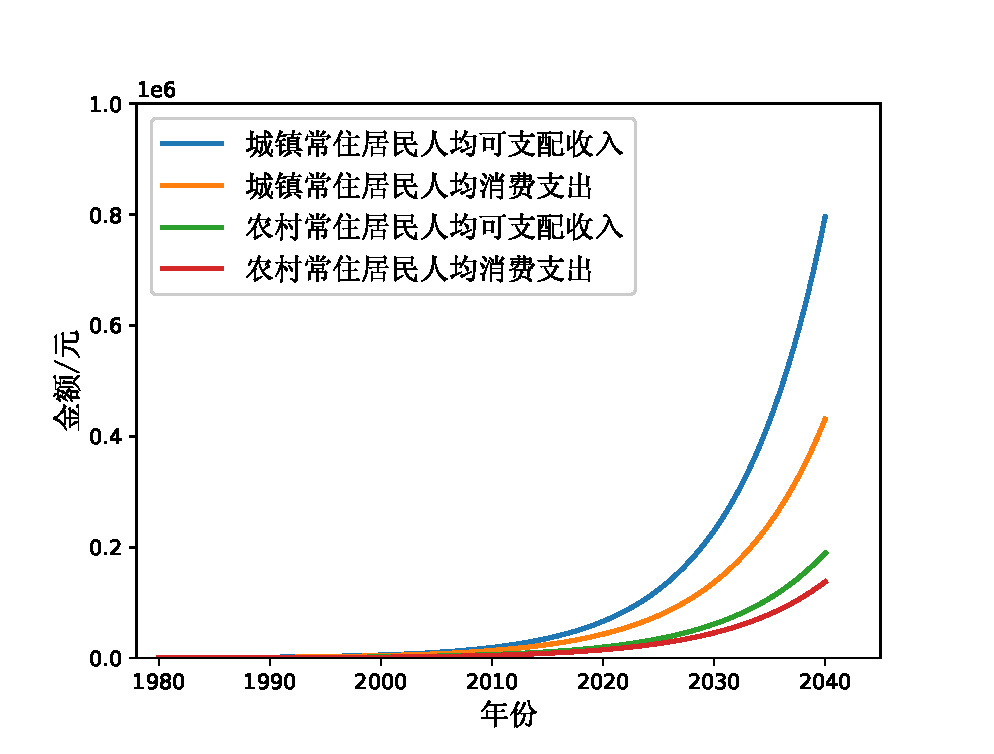
\includegraphics[width=0.8\textwidth]{figures/result1.eps}
  \caption{未来发展趋势}
  \label{fig:side:d}
\end{figure}

\indent 通过对于图 \ref{fig:side:d} 的分析, 可以发现, 未来的发展趋势将会如下所示:
\begin{itemize}
  \item 城镇人均可支配收入和消费支出的差值将会越来越大.
  \item 乡村人均可支配收入和消费支出的差值将会越来越大.
  \item 城镇人均可支配收入和消费支出的差值将会大于乡村人均可支配收入和消费支出的差值.
\end{itemize}

根据模型, 2040 年各项数据均会达到 2020 年的 10 倍左右.\\

\section{问题解答}

\subsection{问题一}

\begin{mdframed}
\fangsong
\textbf{问题 1:} 那么 $5$ 年后 ($2023$ 年)、$10$ 年后 ($2028$ 年) 和 $20$ 年后 ($2038$ 年), 我国居民的人均可支配收入及消费支出分别会达到什么水平?
\end{mdframed}

$5$ 年后 ($2023$ 年), $10$ 年后 ($2028$ 年) 和 $20$ 年后 ($2038$ 年), 我国居民的人均可支配收入及消费支出分别会达到如下表 \ref{tab:2} 水平 (单位: 元).

\begin{table}[H]
  \centering
  \caption{问题 1 未来发展趋势}
  \label{tab:2}
  \begin{tabular}{ccccc}
    \hline
    \textbf{年份} & \textbf{城镇可支配收入} & \textbf{城镇消费支出} & \textbf{乡村可支配收入} & \textbf{乡村消费支出} \\
    \hline
    2023 & $96337.3045$ & $61066.6611$ & $27827.8093$ & $21003.5239$ \\
    2028 & $179276.7357$ & $108507.1504$ & $48936.6133$ & $36505.9487$ \\
    2038 & $620844.4837$ & $342583.7225$ & $151336.5031$ & $110282.4968$ \\
    \hline
  \end{tabular}
\end{table}

\subsection{问题二}

\begin{mdframed}
\fangsong
\textbf{问题 2:} 试评价问题 (1) 中建立的模型效果.
\end{mdframed}

\indent 首先, 从数据角度分析, 表 \ref{tab:1} 中显示, 拟合数据误差率都在 $1\%$ 以左右, 因此模型的拟合效果较好.\\
\indent 其次, 图 \ref{fig:side:d} 和散点图 (见图 \ref{fig:side:c}) 的结果基本相同.\\
\indent 最后, 从模型的角度分析, 通过对于模型的分析, 可以发现, 从 1978 年至 2018 年, 中国居民人均可支配收入和支出主要呈现指数增长的趋势.\\
\indent 但是, 由于指数函数模型的特殊性, 到后期时间越长, 增长速度逐渐呈现爆炸性增长, 因此模型的预测结果可能会出现较大的误差.\\

\subsection{问题三}

\begin{mdframed}
\fangsong
\textbf{问题 3:} 一位同学尝试用二次函数
\begin{equation}
  \label{eq:2}
  h\left(x\right)=\theta_1 x^2+\theta_0
\end{equation}
来拟合 1978 -- 1982 这 5 年的城镇常住居民人均收入可支配,用这个假设函数得到的 2038 年城镇常住居民人均收入可支配为多少? 与 (1) 的效果相比哪一个更好?
\end{mdframed}

首先, 根据要求的二次函数拟合模型, 通过 \texttt{Python} 的 \texttt{sklearn} 库, 笔者得到了如下的结果:

$$
  h\left(x\right) = 384.786207 + 7.902299 * \left(x-1978\right)^2
$$

\indent 其中误差 $loss = 0.65037356$, 误差率为 $0.715\%$.\\
\indent 通过预测, 得到 2038 年城镇常住居民人均收入可支配为 $h\left(2038\right) = 28833.062607$ 元. 然而, 根据数据, 从 2014 年开始, 城镇常住居民人均收入可支配已经超过了 28833 元.\\
\indent 因此, 二次函数模型的预测结果不及笔者所建立模型准确.\\
\end{document}
